\section{Session Date: 8th of January, 2025}
\subsection*{Main Topic: Determinants and Jacobian Determinant, Electromagnetism and Special Relativity}
\subsection*{Topics Covered}
\begin{itemize}
    \item Permutations, \(sgn(\sigma)\) and the symmetric group
    \item Leibniz' formula for the determinant
    \item Contraction of \(\epsilon_{ijk} T^{ij} \) where \(T^{ij}\) is symmetric
    \item Coordinate transformations in integrals and the Jacobian 
    \item Intuition about line integral formula
\end{itemize}

\subsection*{Key Insights}
\paragraph{Permutations and the Symmetric group}
A permutation \(\sigma\) is a bijective (one-to-one) map on a set onto \textit{itself} (which means it just reorders the elements of the set). The collection of all possible permutations of a set is called \textit{the symmetric group} and is denoted with \(S_n\). A common notation is cyclic notation. It is probably best illustrated with an example. Denoting the original set ordering on top and the permuted set on the bottom, let's write the following permutation in cyclic notation\begin{gather*}
    \left\{ 1, 2, 3, 4, 5, 6, 7 \right\} \\
    \downarrow\\
    \left\{ 2, 3, 6, 5, 4, 1, 7\right\}
\end{gather*}  
We can think very algorithmically about this permutation as follows:
\begin{itemize}
    \item 1 is sent to 6
    \item 6 is sent to 3
    \item 3 is sent to 2
    \item 2 is sent to 1
\end{itemize}
\textit{This} is now a closed cycle. In other words, if we continue we just repeat the same cycle. We write the above cycle as \begin{align*}
    \kappa _1 = (1632)
\end{align*}
where the cycle ends before we get back to where we started, such that the string only contains unique numbers. But just because 4 and 5 and 7 do not appear in the above cycle it doesn't mean that they weren't permutated, just that their permutation cycle is \textit{disjoint} from the first one. We see that we also have the disjoint cycle \begin{align*}
    \kappa _2 = (45)
\end{align*}
and the trivial 'cycle' (which by convention is omitted) where 7 is left in its starting position. The complete permutation is thus written as the multiplication of the two sub-permutations. The group multiplication of this group is function composition, that is, first applying one permutation and then applying the next permutation on the result of that first permutation\begin{align*}
    \tau \star \sigma (x_i) = \tau (\sigma (x_i)) = \tau \circ \sigma (x_i)
\end{align*}
where the star is used to show a multiplication as a group operation and the \(\circ \) shows that in this case it is our classical notion of function composition. The advantage of using cycle notation where we identify all disjoint sub-permutation cycles is that since the order of two disjoint cycles obviously doesn't matter, we find that \begin{align*}
    \tau \circ \sigma (x_i) = \sigma \circ \tau (x_i)\qquad \text{if \(\tau\) and \(\sigma\) are disjoint}
\end{align*}
We can thus write the full permutation as\begin{align*}
    \sigma = \kappa_1 \kappa _2 = (1632)(45) = (45)(1632) = \kappa _2 \kappa _1
\end{align*}
where the products are implicit between parantheses.

Any permutation can obviously be represented by succesively interchanging two elements at a time. We call such a switch a \textit{transposition} and often denote it as \(\tau\). We can thus decompose any permutation as \begin{align*}
    \sigma = \tau _1 \tau _2\dots \tau _r
\end{align*} 
The number of transposition used in decomposing a permutation is \textit{not} unique, but it is unique on the equivalence class \(r\) mod 2. We can thus define a unique characteristic/map(?) \begin{align*}
    sgn(\sigma) = (-1)^r = \begin{dcases}
        +1 \quad &\text{if \(r\) is even}\\
        -1 \quad &\text{if \(r\) is odd}
    \end{dcases}
\end{align*}

The reason for introducing all this is the following topic.

\paragraph{Leibniz' determinant formula}
The determinant of a \(3\times3\) matrix is given as follows \begin{align*}
    det(A) = \begin{vmatrix}
        a & b & c\\
        d & e & f\\
        g & h & i
    \end{vmatrix} = aei + bfg + cdh - afh - bdi - cfg
\end{align*} 
We can notice a pattern based on permutations: In each row \(i\) of the matrix, we pick a single column \(j\). This gives us three elements and we multiply these together. Let's say we pick (in order of increasing row index) \(1,3,2\). This would mean that we form the product \begin{align*}
    a_{11}a_{23}a_{32} = afh   
\end{align*}
And now, we count the transpositions needed to permute the column indicies of this set into an ordered (increasing) set (which in the case of an \(n\times n\) matrix is just \(\left\{ 1, \dots , n \right\} \)). Here, we just need a single transposition \begin{align*}
    \sigma = (32) = \tau _1
\end{align*}
But if we had instead started with \(2, 3, 1\) we would have to do \begin{align*}
    \sigma = \tau _1 \tau _2 = (32)(12)
\end{align*} 
Note that permutations in general do not commute unless the are disjoint. Decomposing a permutation into transpositions will in general not only have distinct transpositions of course, since this would imply that the starting permutation already only consisted of disjoint transpositions (or trivial permutations).

If we sum all the possible triplets that can be constructed and let the sign with which they contribute in the sum be determined by whether the number of transpositions needed to permute the triplet into "identity" triplet \(\left\{ 1, 2, 3 \right\} \), we in fact get the determinant! And this sign is \textbf{exactly} what the sign function (funnily enough) gives us! Just go back and check that the determinant for a \(3 \times 3\) works like this. For example, the term \(bdi\) has a negative sign, since \(b\) is in column 2, \(d\) is in column 1 and \(i\) is in column. We thus need a single transposition to do \begin{align*}
    \left\{ 2, 1, 3 \right\} \stackrel{\sigma = (12)}{\longrightarrow} \left\{ 1, 2, 3 \right\} 
\end{align*}
and for this map \begin{align*}
    sgn(\sigma ) = (-1)^1 = -1
\end{align*}

The incredible fact is, that this way of computing the determinant works in \(N\) dimensions! The proof of this is quite technical and relies on understanding multilinear maps (which are tensors in fact). The proof shows that the only possible map that can satisfy all the abstract properties of the determinant is precisely given by the Leibniz' formula (which is the generalisation of the above idea to \(N\) dimensions). It could be fun to revisit when you understand tensors!

Now here comes the formula. Let \(A\) be an \(n \times n\) matrix. Just reading of the description we can write then write the determinant out like this: \begin{align*}
    det(A) = \sum_{\sigma \in S_n} \rm{sgn}(\sigma)a_{1, \sigma (1)}a_{2, \sigma (2)}\dots a_{n, \sigma (n)} 
\end{align*}
How is this the same? Well, let's try working it out in 3 dimensions again. First, we see that we are summing over all \(\sigma \in S_n\). This means all possible permutations we could consider of the set \(\left\{ 1, \dots, n\right\}\), where as before we will interpret the entry index as the row number and the value at that index as the column number. How do we write that more formally? It is just \begin{align*}
    \sigma (i) = j
\end{align*}
to denote that in row \(i\) we pick column enty \(j\) of course!! Note that using only permutations automatically forces us to pick a new column for each row, since otherwise we do not have a bijection (which permutations are defined to be). This is quickly seen if we choose the elements \(aeg\) which has the column indicies \(\left\{ 1, 2, 1 \right\} \). This can never be mapped to \(\left\{ 1, 2, 3\right\}\) by reordering the elements; equivalently, any attempt at constructing such a map \textit{cannot} be injective, since it forces us to map \(1\) onto two different elements (1 and 3).

Lastly, the \(\rm{sgn}(\sigma)\) makes sure that we get the sign correct for the current permutation we are using.

Using product notation we get the usual expression for the Leibniz formula:
\begin{align*}
    \boxed{\text{det}(A) = \sum_{\sigma \in S_n}\left(\text{sgn}(\sigma) \prod_{i=1} ^n a_{i, \sigma (i)}\right)}
\end{align*}
Simply beautiful!

And it get's better than that! Right now we are using permutations and the sign function to only allow unique column indicies as well as keep track of what sign each term should have. But if we notice that "only allowing unique column indicies" is equivalent to saying that any terms with a repeating column index is just set to 0, we see that the exact same result is given by \begin{align*}
    \text{det}(A) &= \sum_{i_1, i_2, \dots, i_n}  \epsilon_{i_1, i_2, \dots, i_n} a_{1, i_1}a_{2, i_2}\dots a_{n, i_n}
\end{align*}
where the sigma is often omitted due to Einstein notation. In other words, the Levi-Civita symbol counts if the number of transpositions needed to get from a permutation to whatever we define as the "identity" permutation is odd or even \textit{while} only allowing actual permutations (by setting things that aren't permutations equal to zero).

Now that we understand this formula, we are ready to use it! But first, we need to note another cool, general identity:
\paragraph{Contraction of \(\epsilon_{ijk} T^{ij} \) where \(T^{ij}\) is symmetric}
This is quite obvious in fact: \begin{align*}
    \epsilon _{ijk} T^{ij} &= \frac{1}{2}\left( \epsilon_{ijk}T^{ij} + \epsilon_{jik}T^{ji}\right) \\
    &= \frac{1}{2}\left( \epsilon_{ijk}T^{ij} - \epsilon_{ijk}T^{ji} \right) \\
    &= \frac{1}{2}\left( \epsilon_{ijk}T^{ij} - \epsilon_{ijk}T^{ij} \right)\\
    &= 0
\end{align*}
In other words \textbf{contracting \(\epsilon _{ijk}\) with a symmetric matrix always gives zero.}

\paragraph{Coordinate transformations in integrals and the Jacobian}
Consider that we want to integrate some function \(f(x,y)\) which represents some density over a region \(g(D)\). That would usually be written as \begin{align*}
    I = \iint_{g(D)} f(x, y) dx dy
\end{align*}
But what does this integral look like in the coordinate system where the region we integrate over is just \(D\)? Say we label the coordinate axes in that system as \((u, v)\). That means that a small region in the \((u, v)\) system is sent to the region \((x,y) = g(u, v)\) and the value of the density function goes from \(f(g(u, v)) \to f(x,y)\). In other words, the values that \(f\) take on will not change, only the label which we give those points. But the are of out integration region \textit{does} change. To make sure that the result we get from integrating using a different coordinate system, we need to make sure that we scale the area of the original disk \(D\) by an appropriate amount to make sure the integrals are equal. This appropiate amount can be different at each small region \(dudv\) throughout \(D\). It turns out to be given by the (absolute value of the) determinant of the Jacobian at the point
\begin{align*}
    \text{abs}|\mathbf{J}|(u, v) &= \begin{vmatrix}
        \frac{\partial g_1}{\partial u}(u, v) & \frac{\partial g_1}{\partial v}(u, v)\\
        \frac{\partial g_2}{\partial u}(u, v) & \frac{\partial g_2}{\partial v} (u, v) 
    \end{vmatrix}\\
    &= \frac{\partial g_i}{\partial x_j}\Biggr|_{(u, v)}
\end{align*}  to make sure that \begin{align*}
    \iint_{g(D)} f(x, y) dx dy = \iint_D f(g(u, v)) \text{abs}|\mathbf{J}| du dv
\end{align*}

It is probably best illustrated by the following image (credit to Mathemaniac on YouTube):
\begin{figure}[h]
    \centering
    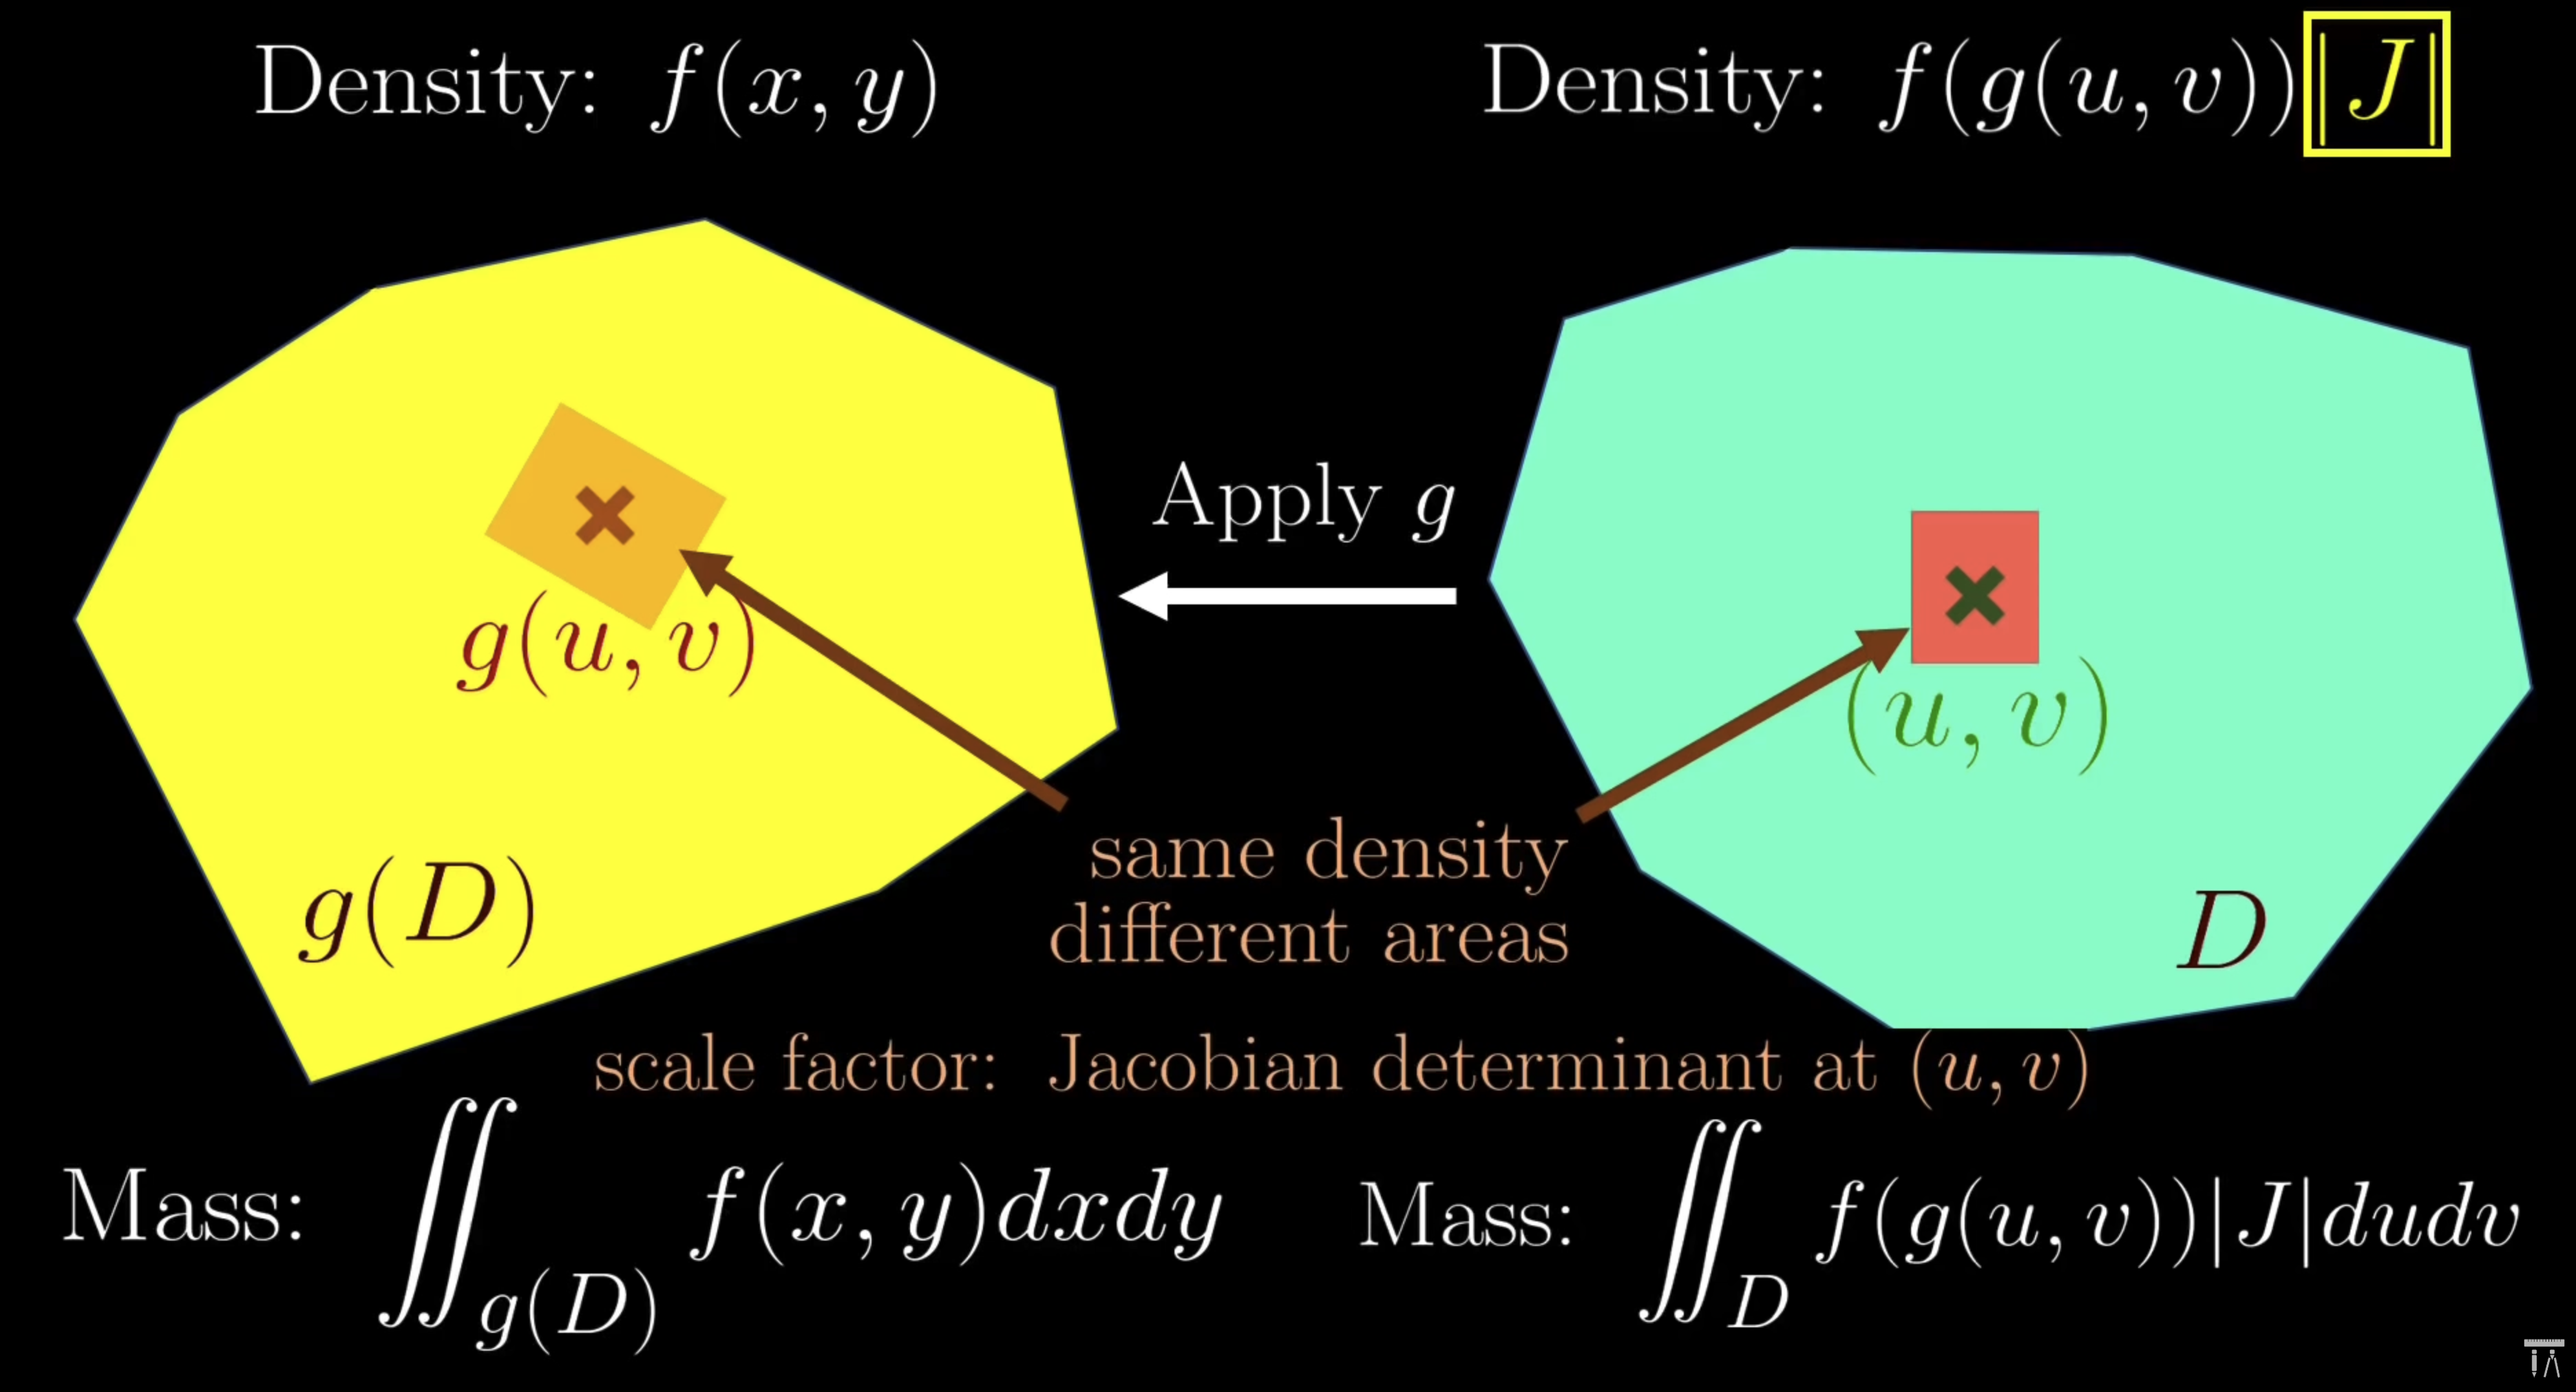
\includegraphics[width=1\textwidth]{Jacobian_intuition.png}
\end{figure}

\paragraph{Liénard-Wiechert Potentials Derivation}
Finally we are able to use the above ideas to derive the Liénard-Wiechert potentials (again!) in a cool way. From Griffith's we end with the conclusion that for a moving point charge, any volume element (no matter the size) is transformed as \begin{align*}
    d \tau ^{\prime} \to \frac{d \tau}{1 - \hatgriffr \cdot \mathbf{v}/c}
\end{align*}
where the \(d \tau ^{\prime} \) is the apparent volume (the one an observer looking at the volume element) sees, whereas \(d \tau \) is the actual volume element if the particle were moving with the same uniform velocity as the observer. 

Here comes the clever thinking: if this is the case, then that must mean that there should be some coordinate transformation which introduces the scaling factor as the absolute value of a Jacobian matrix! In other words, we should be able to find
\begin{align*}
   \vert \text{det}(\mathbf{J})\vert = \frac{1}{1 - \hatgriffr \cdot \mathbf{v}/c}
\end{align*}
for some map. An obvious candidate is the term in the delta function \begin{align*}
    V(\mathbf{r}, t) = \frac{1}{4\pi\epsilon_0} \int \frac{\delta ^3 (\mathbf{r}^{\prime} - \mathbf{w}(t_r))}{}
\end{align*}

\subsection*{Problems Attempted}
\begin{enumerate}
    \item \textit{Problem statement or reference.}
    \item \textit{Solution (include partial work if needed).}
\end{enumerate}

\subsection*{Follow-Up Questions/Ideas/ToDos}
\begin{itemize}
    \item Rewatch the Mathemaniac video to understand the Jacobian better as an approximation of a linear map
\end{itemize}
